\subsection{Generative Adversarial Networks}
Generative modeling is an unsupervised learning approach (Sec.~\ref{sec:nn-training}). A generative model takes a set of training examples and learns the probability distribution that produced them. GANs are generative models first introduced by \textcite{goodfellowGenerativeAdversarialNetworks2014}.
GANs have been particularly successful in image and video generation. They have also been used to create synthetic data, for training other machine learning models and to fill in gaps in missing data \parencite{goodfellowGenerativeAdversarialNetworks2020}.

\subsubsection{Basic Generative Adversarial Networks}\label{sec:basic-gan}

GANs are based on game theory, which studies situations where several decision-makers are present. Each participant chooses an action, and the outcome depends on the choices of all participants. A GAN has two decision-makers, the generator $G$ and the discriminator $D$, typically implemented as neural networks. $G$ takes a vector of random noise as input and generates a sample as output. $D$ takes a real or generated data sample as input and outputs a probability that the input sample is real. The goal of $G$ is to fool $D$ by generating realistic samples. The goal of $D$ is to distinguish real samples from generated ones.

Assume that the data $x$ follows an unknown distribution $p_{data}$, from which new samples need to be generated. The generator is a neural network $G(z; \theta_g)$, where $\theta_g$ denotes the learnable parameters. The input $z$ is a noise vector drawn from a prior distribution $p_z$. Gaussian distribution is normally used to define $p_z$; the GAN framework does not add limitations. The probability distribution of the generated samples is denoted $p_g$. The discriminator is a neural network $D(x; \theta_d)$, with learnable parameters $\theta_d$. It outputs the estimated probability that the input was drawn from  $p_{data}$ rather than $p_{g}$. $G$ and $D$ have cost functions, respectively $J^{(G)}(\theta_d, \theta_g)$ and $J^{(D)}(\theta_d, \theta_g)$. Both $G$ and $D$ need to minimize their cost functions, while they can only control their learnable parameters, respectively $\theta_g$ and $\theta_d$. Hence, the solution is a Nash equilibrium, rather than a minimum of a single cost function.

The GAN framework is flexible in the sense of the cost functions applied to $G$ and $D$. The simplest version of the game is a zero-sum game. In this, the sum of all of the cost functions is always zero.
\begin{equation}
J^{(G)}(\theta_d, \theta_g) = -J^{(D)}(\theta_d, \theta_g).
\end{equation}

The cost function of $D$ is defined as a standard cross-entropy (Sec.~\ref{sec:nn-training})
\begin{equation}
J^{(D)}\bigl(\theta_d, \theta_g\bigr)
= -\frac{1}{2}\,\mathbb{E}_{x \sim p_{\text{data}}} \log D(x)
  - \frac{1}{2}\,\mathbb{E}_{z} \log\bigl(1 - D\bigl(G(z)\bigr)\bigr).
\end{equation}

Learning the zero-sum game minimizes the Jensen-Shannon divergence between $p_{\mathrm{data}}$ and $p_g$. Convergence holds only if both players are updated in function space. In function space $D$ and $G$ are updated freely among all possible functions. In practice, $D$ and $G$ are neural networks and updated in parameter space. In parameter space the reachable functions are limited to those the network architecture can represent. $D$ minimizes a cross-entropy while $G$ maximizes the same quantity. Generated samples are rejected with high confidence at the start of training, and the gradient of $G$ vanishes at the point at which it performs worst \parencite{goodfellowNIPS2016Tutorial2017}.

Therefore, the cost function of $G$ is constructed by flipping the target of the cross-entropy.

\begin{equation}
J^{(G)}(\theta_d, \theta_g)
= -\frac{1}{2}\,\mathbb{E}_{p_{z}}
  \bigl[\log[D(G(z;\theta_g);\theta_d)]\bigr].
  \label{eq:generator-cross}
\end{equation}

The cost function of $D$ and $G$ do not sum to zero anymore, hence the game is no longer zero-sum. Alternative cost functions have been introduced over time.

Fig.~\ref{fig:standard-gan} is the visualization of a standard GAN workflow adapted from \textcite{vuleticFinGANForecastingClassifying2024}.

\begin{figure}[htbp]
    \centering
    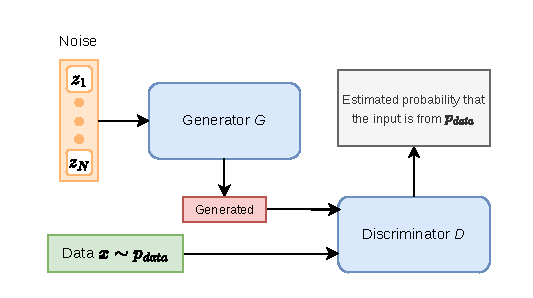
\includegraphics[width=0.7\textwidth]{figures/basic_gan.pdf}
    \caption{Structure of a standard GAN}
    \label{fig:standard-gan}
\end{figure}

GANs are trained by updating the two networks in turn. At each step, a minibatch of samples and noise vectors are drawn from $p_{\mathrm{data}}$ and $p_z$ respectively. $D$ is updated with respect to $\theta_d$ while $\theta_g$ is fixed. $G$ is updated with respect to $\theta_g$ while $\theta_d$ is fixed. $D$ is commonly trained $k$ times for every update of $G$, although \textcite{goodfellowNIPS2016Tutorial2017} argues that $k=1$ is sufficient. $k$ is defined as an independent training parameter. The update cycle is shown in Fig.~\ref{fig:gan-update-cycle}.

\begin{figure}[htbp]
    \centering
    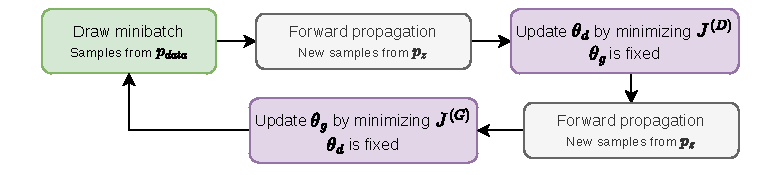
\includegraphics[width=0.9\textwidth]{figures/gan_update_cycle.pdf}
    \caption{Alternating update cycle of a GAN. One $D$ update is performed per $G$ update ($k=1$).}
    \label{fig:gan-update-cycle}
\end{figure}

As stated previously, convergence is not guaranteed in practice. This means that the training of a GAN can settle in a state where $p_g \neq p_{\mathrm{data}}$. The most common such state is mode collapse. It occurs when $G$ repeatedly maps noise vector to very similar outputs. As a result, $p_g$ covers only a small part of $p_{\mathrm{data}}$ but $D$ assigns a high probability that the generated samples are real. Mode collapse is still an unresolved challenge in GAN training. In recent years, several strategies have been proposed to mitigate its effect, such as stronger generators and discriminators, longer training and regularization. However, each of these approaches comes with drawbacks \parencite{barshaIndepthReviewAnalysis2025}.

\subsubsection{cGANs}
Standard GANs can be extended to conditional models \parencite{goodfellowGenerativeAdversarialNetworks2014}. This extension was further developed by \textcite{mirzaConditionalGenerativeAdversarial2014}. In Conditional Generative Adversarial Networks (cGANs), the data follow a conditional distribution $p_{\mathrm{data}}(x \mid \mathrm{c})$, where $c$ is auxiliary deterministic information. The condition is applied to $D$ and $G$ as an additional input.
The cost functions for $G$ and $D$ are the same as for a standard GAN with the condition $c$.

\begin{equation}
J^{(D)}\bigl(\theta_d, \theta_g\bigr)
= -\frac{1}{2}\,\mathbb{E}_{x \sim p_{\text{data}}} \log D(x\mid c)
  - \frac{1}{2}\,\mathbb{E}_{z} \log\bigl(1 - D\bigl(G(z\mid c)\bigr)\mid c\bigr).
\end{equation}

Fig.~\ref{fig:cgan} is the visualization of a cGAN workflow adapted from \textcite{vuleticFinGANForecastingClassifying2024}.

\begin{figure}[htbp]
    \centering
    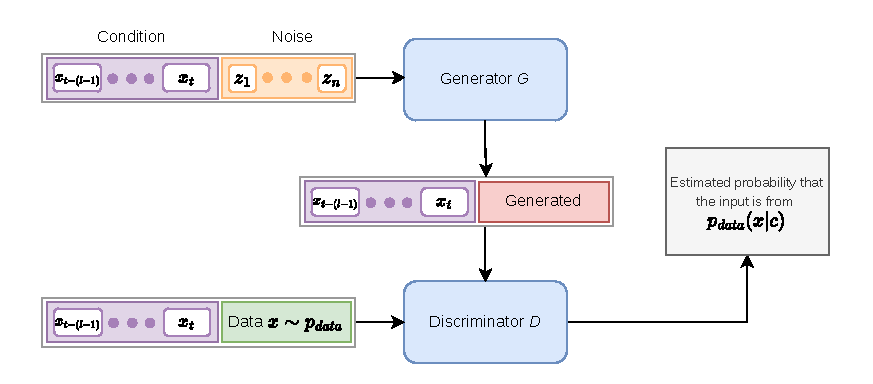
\includegraphics[width=\textwidth]{figures/cgan.pdf}
    \caption{Structure of a cGAN}
    \label{fig:cgan}
\end{figure}


\subsubsection{ForGAN}\label{sec:forgan}
The conditional input proposed in cGANs by \textcite{mirzaConditionalGenerativeAdversarial2014} prepared the ground for domain-specific GAN architectures. ForGAN was introduced specifically for time series forecasting \parencite{koochaliProbabilisticForecastingSensory2019}.

ForGAN is trained to approximate the conditional distribution of the next value in a time series. The condition is the sequence of the previous $l$ observations, ending at time~$t$

\begin{equation}
c = (x_{t-(l-1)}, \ldots, x_t).
\end{equation}

A sliding window of $l+1$ observations is moved along the series. At each position, the first $l$ observations form $c$ and the last is $x_{t+1}$.
$G$ takes a noise vector $z$ and $c$ and outputs a value for the target $x_{t+1}$. $D$ takes a value of $x_{t+1}$ and $c$ and outputs the probability that $x_{t+1}$ is from $p(x_{t+1}\mid c)$. 

A full probabilistic distribution of $x_{t+1}$ can be obtained through repeated sampling of $G$ with different noise vectors and the same $c$.

ForGAN adds a recurrent layer (Sec.~\ref{sec:rnn}) to $G$ and $D$. The layer processes $c$ as an ordered sequence and constructs a vector representation. The recurrent layer can be an LSTM or a GRU (Sec.~\ref{sec:rnn}). The high-level architecture of the ForGAN model is shown in Fig.~\ref{fig:forgan_architecture}.

\begin{figure}[htbp]
  \centering
  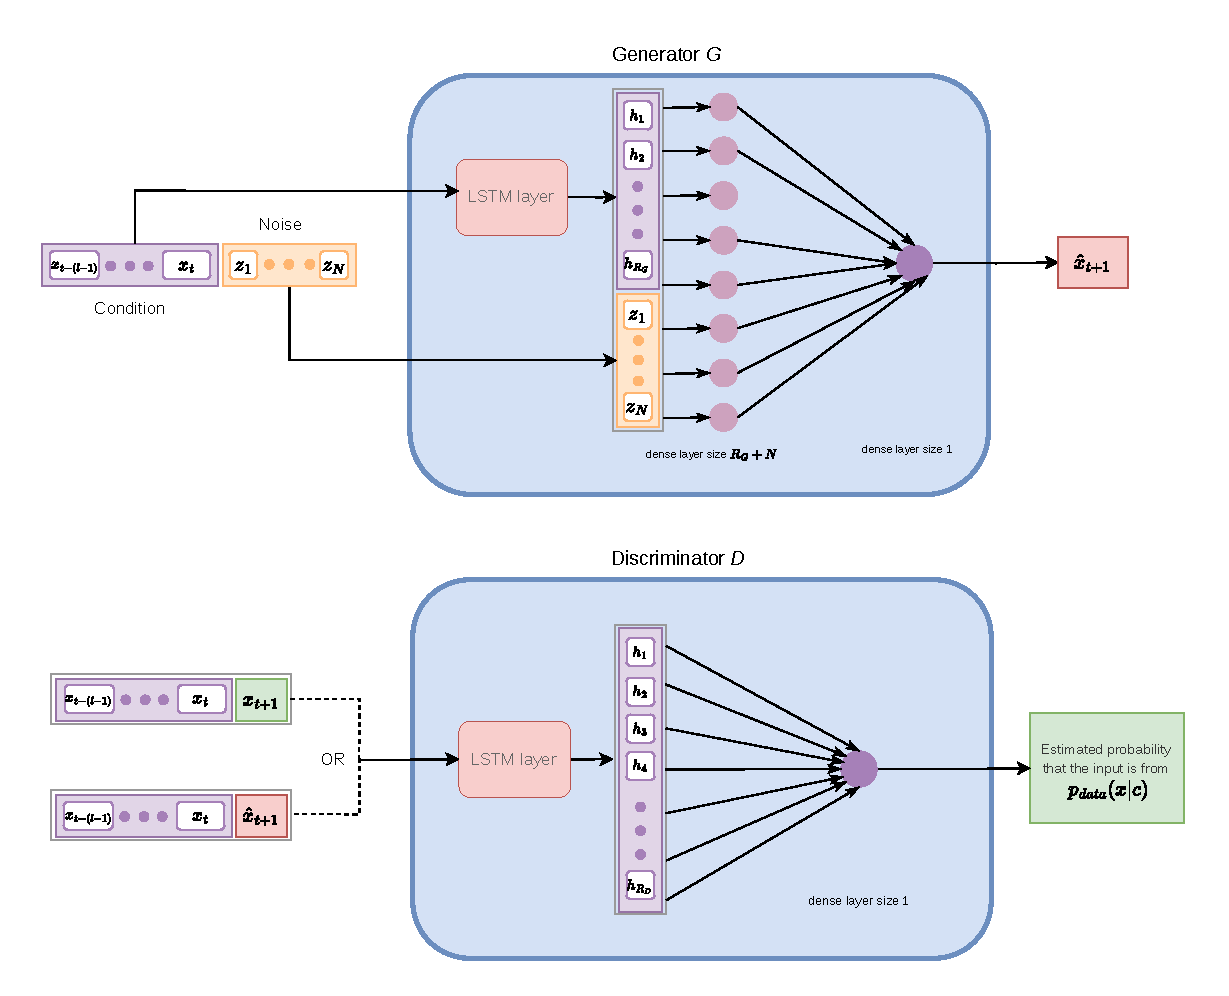
\includegraphics[width=\textwidth]{figures/forgan_architecture.pdf}
  \caption{Structure of a ForGAN}
  \label{fig:forgan_architecture}
\end{figure}

\clearpage
\subsubsection{Fin-GAN}\label{sec:fin-gan}
Fin-GAN was introduced as an extension of ForGAN \parencite{vuleticFinGANForecastingClassifying2024}. It focuses on the probabilistic forecasting of financial time series, specifically equity returns. The ForGAN architecture and the cost function of $D$ are unchanged. LSTM is chosen as the recurrent layer. 

The motivation behind Fin-GAN is to correctly forecast the sign of the return, since the sign determines whether the trade is profitable. For this purpose, economics-driven terms are introduced into the cost function of $G$. In contrast to the unsupervised setting of standard GANs, \textcite{vuleticFinGANForecastingClassifying2024} classify Fin-GAN as supervised learning.

The terms are defined over a minibatch of $n_{\text{batch}}$ pairs. For each condition in the batch, G produces a forecast $\hat{x}_i$ of the realized value $x_i$. Let $\hat{x}=(\hat{x}_1, \ldots, \hat{x}_{n_{\text{batch}}})$ and $x=(x_1, \ldots, x_{n_{\text{batch}}})$. 

\textbf{Cost function.} $J^{(G)}$ can be the zero-sum, cross-entropy or Wasserstein cost function. The latter replaces the Jensen–Shannon divergence between $p_{\mathrm{data}}$ and $p_g$ with the Wasserstein-1 distance \parencite{arjovskyWassersteinGAN2017}. \textcite{vuleticFinGANForecastingClassifying2024} report that the Wasserstein cost function was numerically unstable during training. Hence, $J^{(G)}$ is the cross-entropy cost function given in Eq.~\eqref{eq:generator-cross}. In addition, Fin-GAN introduces four economics-driven terms to the cost function. These are defined below. 

\begin{equation}
L^{G}(x, \hat{x}) = J^{(G)}(x, \hat{x})
- \alpha\,\mathrm{PnL}^{*}_{a}(x, \hat{x})
+ \beta\,\mathrm{MSE}(x, \hat{x})
- \gamma\,\mathrm{SR}^{*}(x, \hat{x})
+ \delta\,\mathrm{STD}(x, \hat{x}).
\label{eq:fingan-loss}
\end{equation}

A positive forecast corresponds to buying an asset, and a negative forecast to selling it short. The profit and loss $\mathrm{PnL}$ of the trade is the sign of the forecast multiplied by the realized return $\mathrm{PnL}(x_i, \hat{x}_i)=\mathrm{sgn}(\hat{x}_i)\cdot x_i$. Since only the sign enters the formula, the outcome does not depend on the magnitude of the forecast. $\mathrm{sgn}(\hat{x}_i)$ is not differentiable, so the standard term $\mathrm{PnL}$ would not provide a gradient for training. A smooth approximation is introduced
\begin{equation}
\mathrm{PnL}^{*}_{a}(x_i, \hat{x}_i) = \tanh(k_{\tanh}\,\hat{x}_i)\,x_i,
\end{equation}

where $k_{\tanh}$ is a hyperparameter that controls the accuracy of the approximation. \textcite{vuleticFinGANForecastingClassifying2024} use $k_{\tanh}=100$, that is large enough to give a close approximation and small enough to maintain strong gradients. 

Although the sign of the forecast is the main interest, forecasting an $\hat{x}_i$ that is close to $x_i$ is also of importance. The mean squared error $\mathrm{MSE}$ measures the squared difference between the forecast and the realized value, averaged over the minibatch.

$\mathrm{SR}^{*}$ is defined as the mean of the $\mathrm{PnL}^{*}_{a}$ series divided by its standard deviation.
\begin{equation}
\mathrm{SR}^{*}(x, \hat{x}) = \frac{\bar{p}}{\sqrt{\dfrac{1}{n_{\text{batch}}} \sum_{i=1}^{n_{\text{batch}}} \left( p_i - \bar{p} \right)^{2}}},
\label{eq:sharpe-ratio}
\end{equation}

where $p_i = \mathrm{PnL}^{*}_{a}(x_i, \hat{x}_i)$ and $\bar{p}$ is its mean over the $n_{\mathrm{batch}}$ forecasts. $\mathrm{SR}^{*}$ deviates from Eq.~\ref{eq:std-sharpe-ratio}. The risk-free rate is not subtracted, since the daily risk-free rate is small relative to the daily $\mathrm{PnL}^*_a$. The ratio is not annualized, because a constant factor would be absorbed by the weight $\gamma$ during gradient matching. Lastly, $\mathrm{SR}^*$ is computed over the $n_{\mathrm{batch}}$ forecasts of a minibatch rather than over a return series. As described in Sec.~\ref{sec:nn-training}, SGD requires random minibatches. As a result, forecasts entering $\mathrm{SR}^*$ are not in chronological order \parencite[11]{vuleticFinGANForecastingClassifying2024}.

The standard deviation $\mathrm{STD}$ term is the denominator of Eq.~\ref{eq:sharpe-ratio}. Logically maximizing $\mathrm{SR}^{*}$ is the same as maximizing $\mathrm{PnL}^{*}_{a}$ and minimizing $\mathrm{STD}$ at the same time. As a result, including all three terms in $L^{G}$ is redundant. However, during training $\mathrm{SR}^{*}$ and the combination of $\mathrm{PnL}^{*}_{a}$ and $\mathrm{STD}$ produce different gradients \parencite{vuleticFinGANForecastingClassifying2024}.

\textbf{Gradient matching.} All the terms above are measured in different units, hence they produce incomparable gradients. As a solution, four additional hyperparameters $\alpha$, $\beta$, $\gamma$, $\delta$ are introduced. Fin-GAN is first trained on $J^{(G)}$ only, and gradient norms (Sec.~\ref{sec:nn-training}) of other terms are calculated. Each hyperparameter is the mean of the ratios between the cross-entropy gradient norms and the gradient norms of the corresponding term.
Large values of $\alpha$, $\beta$, $\gamma$, $\delta$ make the feedback of $D$ insignificant and move the model towards supervised learning, but small values leave it in the standard GAN setting.

If the term is not included in the objective, the hyperparameter is set to zero. Several versions of $L^{G}$ can be constructed from different combinations of terms. Only combinations that include economics-driven terms are considered for Fin-GAN. \textcite{vuleticFinGANForecastingClassifying2024} train eight such versions and select the combination with the highest Sharpe ratio $\mathrm{SR}_{w}$ on the validation set. Then, the selected $G$ is evaluated on the test set.

\textbf{Mode collapse.} \textcite{vuleticFinGANForecastingClassifying2024} distinguish two types of mode collapse for time series. Distributional mode collapse happens 
when $G$ generates nearly identical samples for a single condition. 
Mean mode collapse happens when the means of the generated
distributions are nearly identical across all conditions.
Both are identified by a standard deviation below a threshold $\epsilon=0.0002$. Fin-GAN uses normal Xavier initialization (Sec.~\ref{sec:nn-training}), since ForGAN suffered mode collapse in \SI{67}{\percent} of runs under He initialization. However, no mode collapse happened with the economics-driven terms, under either initialization. Mode collapse is a known failure mode of GAN training in general, as described in Sec.~\ref{sec:basic-gan}. 

\textbf{Weighted strategy.} The Sharpe ratio $\mathrm{SR}_{w}$ is not to be confused with the
$\mathrm{SR}^{*}$ term of Eq.~\ref{eq:sharpe-ratio}. $\mathrm{SR}_{w}$
is computed over a full data split on $\mathrm{wPnL}$. $\mathrm{SR}_{w}$ measures the directional accuracy of the forecasts and not the shape of the generated distribution. For each condition, $B$ samples are drawn from $G$ with different noise vectors. 

\begin{equation}
    \label{eq:wpnl-trade}
    \mathrm{wPnL}^{i}_{2} = 10000 \left( p^{i}_{u} - p^{i}_{d} \right) x_i ,
\end{equation}

where $p^{i}_{u}$ and $p^{i}_{d}$ are the fractions of non-negative and negative samples. \textcite{vuleticFinGANForecastingClassifying2024} use $B = 1000$. Since the equity data uses two returns per day, intraday and overnight, two positions are taken per day. The $\mathrm{wPnL}^{i}$ series is 
the sum of the two $\mathrm{wPnL}^{i}_{2}$ values per day. 
For the equity data of \textcite{vuleticFinGANForecastingClassifying2024}, two returns per day give $n_{\text{days}} = \lfloor n/2 \rfloor$. The Sharpe ratio $\mathrm{SR}_{w}$ is then
\begin{equation}
    \label{eq:sharpe-weighted}
    \mathrm{SR}_{w} = \sqrt{252} \,
    \frac{\overline{\mathrm{wPnL}}}
         {\sqrt{\dfrac{1}{n_{\text{days}}}
          \sum_{i=1}^{n_{\text{days}}}
          \left( \mathrm{wPnL}^{i} - \overline{\mathrm{wPnL}} \right)^{2}}},
\end{equation}
where $\overline{\mathrm{wPnL}}$ is the mean of the $\mathrm{wPnL}^{i}$ series over the $n_{\text{days}}$ trading days. The factor $\sqrt{252}$ annualizes the ratio, where 252 is the conventional number of trading days in a year.